\appendix
\section{详细的估计量推导}
\label{app:theory}

正文给出了估计量、其无偏性恒等式以及统一的方差分析。附录提供了详细的 Top-$k$ 偏差推导和单控制预言机计算，包括完整粗粒度分布的边界项抵消。

\subsection{三种有偏的 Teacher \texorpdfstring{Top-$k$}{Top-k} 反向 KL}
\label{app:topk-bias}

本小节区分了三种常被混淆的操作：
在头部对两个分布进行重归一化、截断标量反KL目标，以及仅截断停止系数的梯度。每种操作均可从教师模型的 Top-$k$ 中计算得出，但它们均无法准确估计完整词表反KL目标的梯度。此处的“偏差”是相对于该目标梯度而言的，而非蒙特卡罗采样偏差。固定支持集 $S$ 与教师概率，
令 $z$ 为无限制的学生Logit，定义
\begin{equation}
 \begin{gathered}
 R\coloneqq\sum_i p_i r_i=\KL(p\|q),\qquad
 R_S\coloneqq\sum_{i\in S}p_i r_i,\\
 P\coloneqq\sum_{i\in S}p_i,\qquad
 Q\coloneqq\sum_{i\in S}q_i.
 \end{gathered}
\end{equation}
确切的完整rKL Logit梯度，作为以下参考：
\begin{equation}
 [\nabla_z R]_j=p_j(r_j-R).
 \label{eq:full-rkl-logit-gradient}
\end{equation}

\paragraph{重规范化Top-$k$ 反向KL。}
定义 $\widetilde p_i=p_i/P$ 、$\widetilde q_i=q_i/Q$ 和 $\widetilde r_i=\log(\widetilde p_i/\widetilde q_i)$ 为 $i\in S$，其中包含 $\widetilde R=\sum_{i\in S}\widetilde p_i\widetilde r_i$。由于 $\widetilde p_i=\exp (z_i)/\sum_{\ell\in S}\exp (z_\ell)$，目标函数及其 Logit 梯度为
\begin{equation}
 \begin{aligned}
 L_{\mathrm{renormalized}}
 &=\sum_{i\in S}\widetilde p_i
   \log\frac{\widetilde p_i}{\widetilde q_i},\\
 [\nabla_z L_{\mathrm{renormalized}}]_j
 &=\ind\{j\in S\}\widetilde p_j
   (\widetilde r_j-\widetilde R).
 \end{aligned}
 \label{eq:renorm-topk-gradient}
\end{equation}
每个尾部Logit分量恰好为零，而  
公式~(\ref{eq:full-rkl-logit-gradient}) 在此处通常不为零。全局最小值是集合
\begin{equation}
 \widetilde p_i=\widetilde q_i
 \quad(i\in S)
 \quad\Longleftrightarrow\quad
 p_i=\frac{P}{Q}q_i\quad(i\in S),
 \label{eq:renorm-topk-optimum}
\end{equation}
具有任意的 $P$  和任意的尾部形状。因此，重规范化仅学习条件头部分布；它既无法确定头部质量，也无法识别被省略的条件分布。

\paragraph{标量截断的Top-$k$ 反向KL。}
未规范化的标量捷径为
$L_{\mathrm{truncated}}=R_S=\sum_{i\in S}p_i r_i$ 。写作
$C_S\coloneqq\sum_{i\in S}p_i(r_i+1)=R_S+P$ ，直接微分可得
\begin{equation}
 \begin{aligned}
 \nabla_\theta L_{\mathrm{truncated}}
 &=\bhead+\nabla_\theta P,\\
 [\nabla_z L_{\mathrm{truncated}}]_j
 &=\ind\{j\in S\}p_j(r_j+1)-p_jC_S.
 \end{aligned}
 \label{eq:scalar-truncated-gradient}
\end{equation}
因此，其相对于完整rKL的偏差为
$\nabla_\theta P-\tau_p\bmean_{\mathrm{tail}}$ 。特别是，当
$j\notin S$ ，$[\nabla_z L_{\mathrm{tr}}]_j=-p_jC_S$ ；当 $C_S>0$ 时，
梯度下降会增加每一个被省略的Logit。

相应的全局最优解使失效更加明显。对于每个头坐标，
\begin{equation}
 x\log\frac{x}{q_i}\geq-\frac{q_i}{e},
 \qquad\text{with equality iff }x=\frac{q_i}{e}.
\end{equation}
由于 $\sum_{i\in S}q_i/e=Q/e<1$，所有坐标极小值联合可行，因此
\begin{equation}
 p_i^\star=\frac{q_i}{e}\quad(i\in S),\qquad
 P^\star=\frac{Q}{e},\qquad
 \sum_{j\notin S}p_j^\star=1-\frac{Q}{e},
 \label{eq:scalar-truncated-optimum}
\end{equation}
在尾部内部具有任意分配。即使 $Q$  接近一，此目标也更倾向于在教师头部之外保留大约 $1-1/e$  的学生质量；因此，尾部推动是一种目标层面的特性，而不仅仅是瞬时梯度符号。

\paragraph{停止系数的Top-$k$ 反向KL梯度。}
停止对系数的调整会消除 $\nabla P$ 边界项，但会使尾部期望保持未校正状态：
\begin{equation}
  \begin{gathered}
    \bgrad_{\text{Top-}k} \coloneqq \sum_{i \in S} \operatorname{stopgrad}(p_i r_i) \bscore_i = \bhead, \\
    [\bgrad_{\text{Top-}k}]_j = \ind\{j \in S\} p_j r_j - p_j R_S, \qquad
    \bgrad_{\text{Top-}k} - \bgrad = -\tau_p \bmean_{\mathrm{tail}}.
  \end{gathered}
  \label{eq:stopped-topk-gradient-bias}
\end{equation}
在无限制的类别Logit空间中，若尾部非空，则梯度消失（$\bgrad_{\text{Top-}k} = \mathbf{0}$）迫使 $R_S = 0$ 通过尾部组件（$j \notin S$），这随后意味着对所有头部组件（$i \in S$）有 $r_i = 0$。因此，$p_i = q_i$ 在头部成立，正确匹配了整体尾部质量（$1 - P = 1 - Q$）；然而，尾部上的条件分布仍不受约束且任意。尽管这种停梯度公式在三种启发式方法中对潜在目标的影响最小，但只要尾部向量非零，它仍具有内在的有偏性。HETS 和 ResOPD 通过引入采样尾部修正来恢复缺失的期望，从而解决这一残余偏差。

\subsection{单控制残差化及其方差最优}
\label{app:single-control}

使用公式~(\ref{eq:head-tail-definitions}) 的头/尾记号，令
$J=\ind\{A\notin S\}$ ，并令 $\bm B$ 为任意在采样 $A\sim p$ 之前停止的有限前缀可测向量。考虑单控制估计量
\begin{equation}
 \widehat{\bgrad}(\bm B)
 \coloneqq
 \bhead+\tau_p\bm B+J(\btoken_A-\bm B).
 \label{eq:single-control-estimator}
\end{equation}
它对每一个这样的 $\bm B$ 都是无偏的：
\begin{equation}
 \E[\widehat{\bgrad}(\bm B)]
 =\bhead+\tau_p\bm B
  +\tau_p(\bmean_{\mathrm{tail}}-\bm B)
 =\bgrad.
 \label{eq:single-control-unbiased}
\end{equation}
在给定 $J=0$ 的条件下，其值为确定性向量
$\bhead+\tau_p\bm B$ 。在给定 $J=1$ 的条件下，其均值为
$\bhead+\tau_p\bm B+\bmean_{\mathrm{tail}}-\bm B$ ，协方差为
$\Cov_{\mathrm{tail}}(\btoken_A)$ 。两个条件均值之差为
$\bmean_{\mathrm{tail}}-\bm B$ 。因此，全协方差定律给出
\begin{equation}
 \mathcal V(\widehat{\bgrad}(\bm B))
 =\tau_p\mathcal V_{\mathrm{tail}}(\btoken_A)
 +P\tau_p\lVert\bmean_{\mathrm{tail}}-\bm B\rVert_2^2.
 \label{eq:single-control-variance}
\end{equation}
第一项与 $\bm B$ 无关。因此，每当
$0<P<1$ 时，唯一的迹-协方差最小化器及其确切遗憾为
\begin{equation}
 \begin{aligned}
 \bm B^\star&=\bmean_{\mathrm{tail}},\\
 \mathcal V(\widehat{\bgrad}(\bm B))
 -\mathcal V(\widehat{\bgrad}(\bmean_{\mathrm{tail}}))
 &=P\tau_p\lVert\bm B-\bmean_{\mathrm{tail}}\rVert_2^2.
 \end{aligned}
 \label{eq:single-control-oracle}
\end{equation}
该预言机消除了所有头对尾事件的方差，但在稀疏教师接口下不可用，因为它需要完整的条件尾部均值。

HETS和ResOPD是两种载荷兼容的选择
\begin{equation}
 \widehat{\bgrad}^{\mathrm{HETS}}=\widehat{\bgrad}(\bm 0),
 \qquad
 \widehat{\bgrad}^{\mathrm{ResOPD}}=\widehat{\bgrad}(\bmean_B).
\end{equation}
它们相对于单控制预言机的遗憾分别是
$P\tau_p\lVert\bmean_{\mathrm{tail}}\rVert_2^2$  和
$P\tau_p\lVert\bmean_{\mathrm{tail}}-\bmean_B\rVert_2^2$ 。相减得
\begin{equation}
  \mathcal{V}(\widehat{\bgrad}^{\mathrm{HETS}}) - \mathcal{V}(\widehat{\bgrad}^{\mathrm{ResOPD}}) = P\tau_p \!\left( 2\langle\bmean_{\mathrm{tail}}, \bmean_B\rangle - \lVert\bmean_B\rVert_2^2 \right).
  \label{eq:hets-cfr-variance-appendix}
\end{equation}
因此，确切地当 $\bmean_B$ 比 HETS 对照 $\bm 0$ 更接近 $\bmean_{\mathrm{tail}}$ 时，ResOPD 具有更低的迹协方差；不断言无条件排序。

仍需验证为何在没有精细教师尾部的情况下 $\bmean_B$ 仍然可用。对 $k$  head token 和一个 tail 桶的完整粗粒度分布的反向 KL 为
\begin{equation}
 L_{\mathrm{coarse}}
 \coloneqq
 \sum_{i\in S}p_i\log\frac{p_i}{q_i}
 +\tau_p\log\frac{\tau_p}{\tau_q}.
\end{equation}
由于
$\nabla\tau_p=\tau_p\bar{\bscore}_{\mathrm{tail}}=-\nabla P$ ,
直接微分
可得
\begin{equation}
 \begin{aligned}
 \nabla L_{\mathrm{coarse}}
 &=\bhead+\nabla P+(b+1)\nabla\tau_p\\
 &=\bhead+b\nabla\tau_p
  =\bhead+\tau_p\bmean_B
  =\bgrad_{\mathrm{coarse}}.
 \end{aligned}
\end{equation}
边界项相互抵消，因为尾部伪token完成了粗粒度支持。这就是为什么 $\bgrad_{\mathrm{coarse}}$ 是一个确切的梯度（但有偏），即使 $\bmean_B$ 未必等于真实的条件细粒度尾部均值。

\FloatBarrier
\section{详细的训练和评估配置}
\label{app:hyperparameters}


表格。~\ref{tab:opd-hyperparameters} 和 ~\ref{tab:qwen3-opd-hyperparameters} 收集了主数学领域和跨领域运行的完整情景设置。它们的采样假设在第~\ref{subsec:evidence} 和 ~\ref{sec:ex-setup} 节中进行了讨论；匹配的全支撑数学消融结果在第~\ref{sec:rollout-ablation} 节中报告。

\begin{table}[t]
\caption{\textbf{主数学OPD实验配置和超参数。}}
\label{tab:opd-hyperparameters}
\centering
\small
\renewcommand{\arraystretch}{1.18}
\setlength{\tabcolsep}{6pt}
\begin{tabular}{@{}lll@{}}
\toprule
\textbf{Category} & \textbf{Hyperparameter} & \textbf{Configuration / Value} \\
\midrule

\multirow{2}{*}{\textbf{Models}}
& Student model & Qwen3.5-4B \\
& Teacher model & Qwen3.5-27B \\
\midrule

\multirow{2}{*}{\textbf{Data}}
& Training dataset & 1{,}024 prompts sampled from DeepMath-103K \\
& Max prompt length & 2{,}048 \\
\midrule

\multirow{5}{*}{\textbf{Sampling}}
& Enable thinking & True \\
& Max response length & 32{,}768 (training and evaluation) \\
& temperature & 1.0 \\
& top-$p$ & 0.95 \\
& top-$k$ & 20 \\
\midrule

\multirow{5}{*}{\textbf{Training}}
& Training epochs & 3 \\
& Global batch size & 16 \\
& Optimizer & AdamW \\
& Gradient clipping & 1.0 \\
& Learning rate & $1\times10^{-6}$ \\
\midrule

\multirow{4}{*}{\textbf{System \& Hardware}}
& Compute infrastructure & $16\times$ NVIDIA H200 GPUs \\
& Resource allocation & 8 GPUs for Student rollout, 4 for Student training, \\
& & 4 for hosting the Teacher inference service \\
& Software frameworks & Training: verl \quad Inference: vLLM \\
\bottomrule
\end{tabular}
\end{table}


\section{逐步评估结果}

\subsection{数学运算能力发展实验}
\label{app:math-learning-trajectories}

\begin{table}[t]
\caption{\textbf{跨领域Qwen3 OPD实验配置与超参数。}}
\label{tab:qwen3-opd-hyperparameters}
\centering
\small
\renewcommand{\arraystretch}{1.18}
\setlength{\tabcolsep}{6pt}
\begin{tabular}{@{}lll@{}}
\toprule
\textbf{Category} & \textbf{Hyperparameter} & \textbf{Configuration / Value} \\
\midrule
\multirow{2}{*}{\textbf{Models}}
& Student model & Qwen3-4B \\
& Teacher model & Qwen3-30B-A3B-Instruct-2507 \\
\midrule
\multirow{3}{*}{\textbf{Data}}
& Training dataset & 30,000 deduplicated prompts; \\
& & Math/Code/Science: 10,000 each \\
& Max prompt length & 1,024 \\
\midrule
\multirow{5}{*}{\textbf{Sampling}}
& Enable thinking & False \\
& Max response length & 8192 (training) and 32768 (evaluation) \\
& temperature & 1.0 \\
& top-$p$ & 1.0 \\
& top-$k$ & $-1$ \\
\midrule
\multirow{7}{*}{\textbf{Training}}
& Training steps & 100 \\
& Global batch size & 288 \\
& Optimizer & AdamW \\
& Gradient clipping & 1.0 \\
& Peak learning rate & $5\times10^{-6}$ \\
& LR schedule & 10-step warmup; \\
& & cosine decay to $0.1\times$ peak \\
\midrule
\multirow{4}{*}{\textbf{System \& Hardware}}
& Compute infrastructure & $16\times$ NVIDIA H200 GPUs \\
& Resource allocation & 8 GPUs for student rollout, 4 for student training, \\
& & 4 for hosting the teacher inference service \\
& Software frameworks & Training: verl \quad Inference: vLLM \\
\bottomrule
\end{tabular}
\end{table}


图~\ref{fig:estimator-learning} 展示了在评估套件上的训练轨迹。  
在 DeepMath 的保留集上，ResOPD 显现出稳定的后期增益，在所有估计量中达到了最高的最终准确率。  
尽管像 TA-OPD 和 Teacher Top-$k$  vOPD 这样的竞争性基准表现出持续改进，但在最终检查点处仍不及 ResOPD。与此同时，Sampled-token OPD 在早期达到峰值后严重恶化，而 HETS 则在后期出现下降。  
在外部数学竞赛中也呈现出类似趋势：尽管 TA-OPD 保持了强劲的中期轨迹表现，vOPD 也保持竞争力，但 ResOPD 展现出更优的后期韧性，并在最后一步彻底超越所有其他方法，避免了如 Sampled-token OPD 和 HETS 等估计量所观察到的峰值后退化现象。

结合论文中其他部分报告的固定前缀协方差迹降低和改进的在线训练诊断，这些轨迹与所提出的粗尾残差化方法减少随机梯度噪声并提升后期最优化稳定性一致。

\subsection{跨领域OPD实验}
\label{app:cross-qwen3}

\begin{figure}[t]
\centering
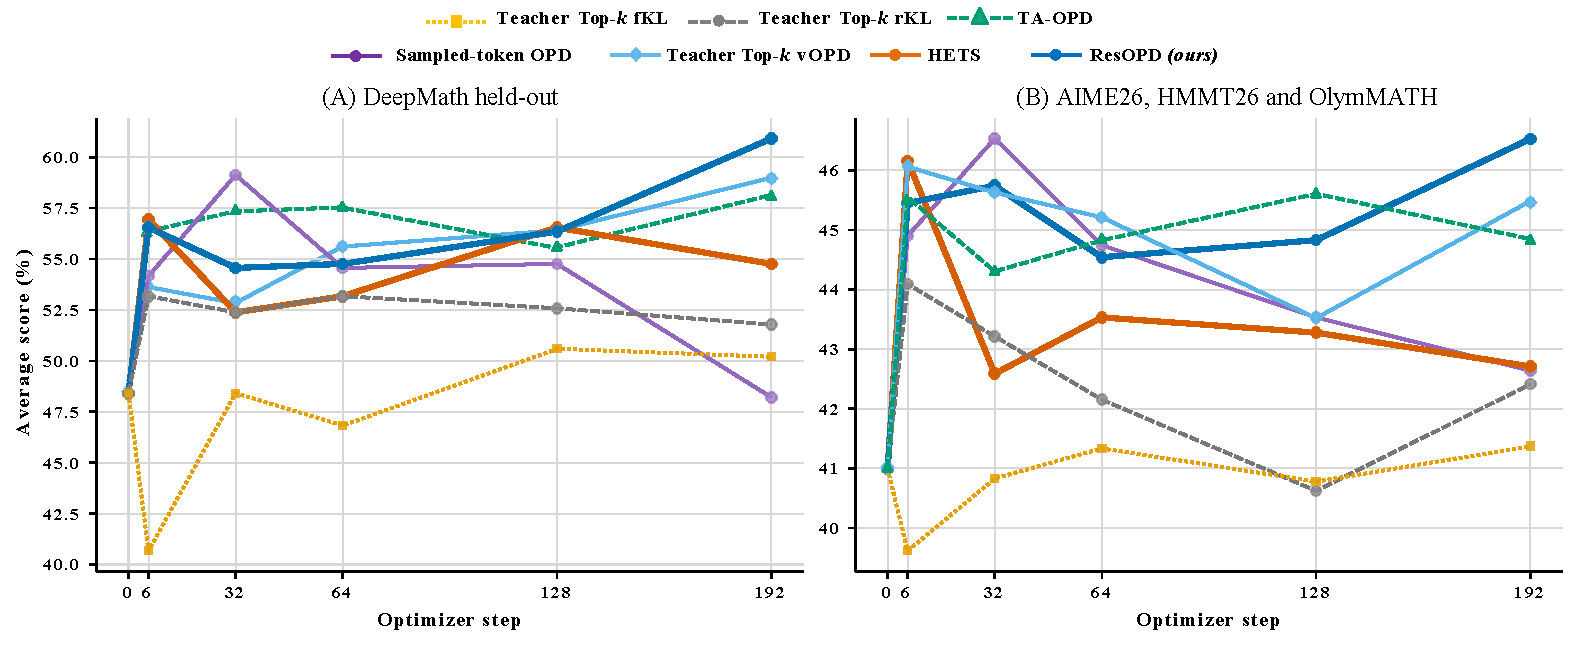
\includegraphics[width=0.85\textwidth]{figs/math_step_v4.pdf}
\caption{\textbf{分步学习曲线} 对应于表~\ref{tab:math-terminal} 在 DeepMath 留出集（左）和外部竞赛（右）上的结果，覆盖 192 个优化器步骤。}
\label{fig:estimator-learning}
\end{figure}

图~\ref{fig:qwen3-transfer-curves} 展示了在所有四个基准上的固定训练进度（步骤 0、10、25、50 和 100）下，检查点评估轨迹。在代码基准（LiveCodeBench v5 和 v6）上，ResOPD 和 HETS 快速收敛，并在整个训练过程中显著优于采样 token 的 OPD，其中 ResOPD 达到了最高的整体轨迹 AUC。相比之下，科学基准表现出混合的领域动态：在 GPQA-D 上，采样 token 的 OPD 展现了更优的保留能力和最终准确率；而 ResOPD 在整个训练步骤中保持竞争力，并在 SuperGPQA 上取得了最佳终端性能。这些轨迹证实，尽管采样 token 的 OPD 在专业科学推理任务中表现强劲，但 ResOPD 在代码任务上提供了良好的迁移性能，同时不牺牲整体多领域平衡性。

\begin{figure}[htbp]
  \centering
  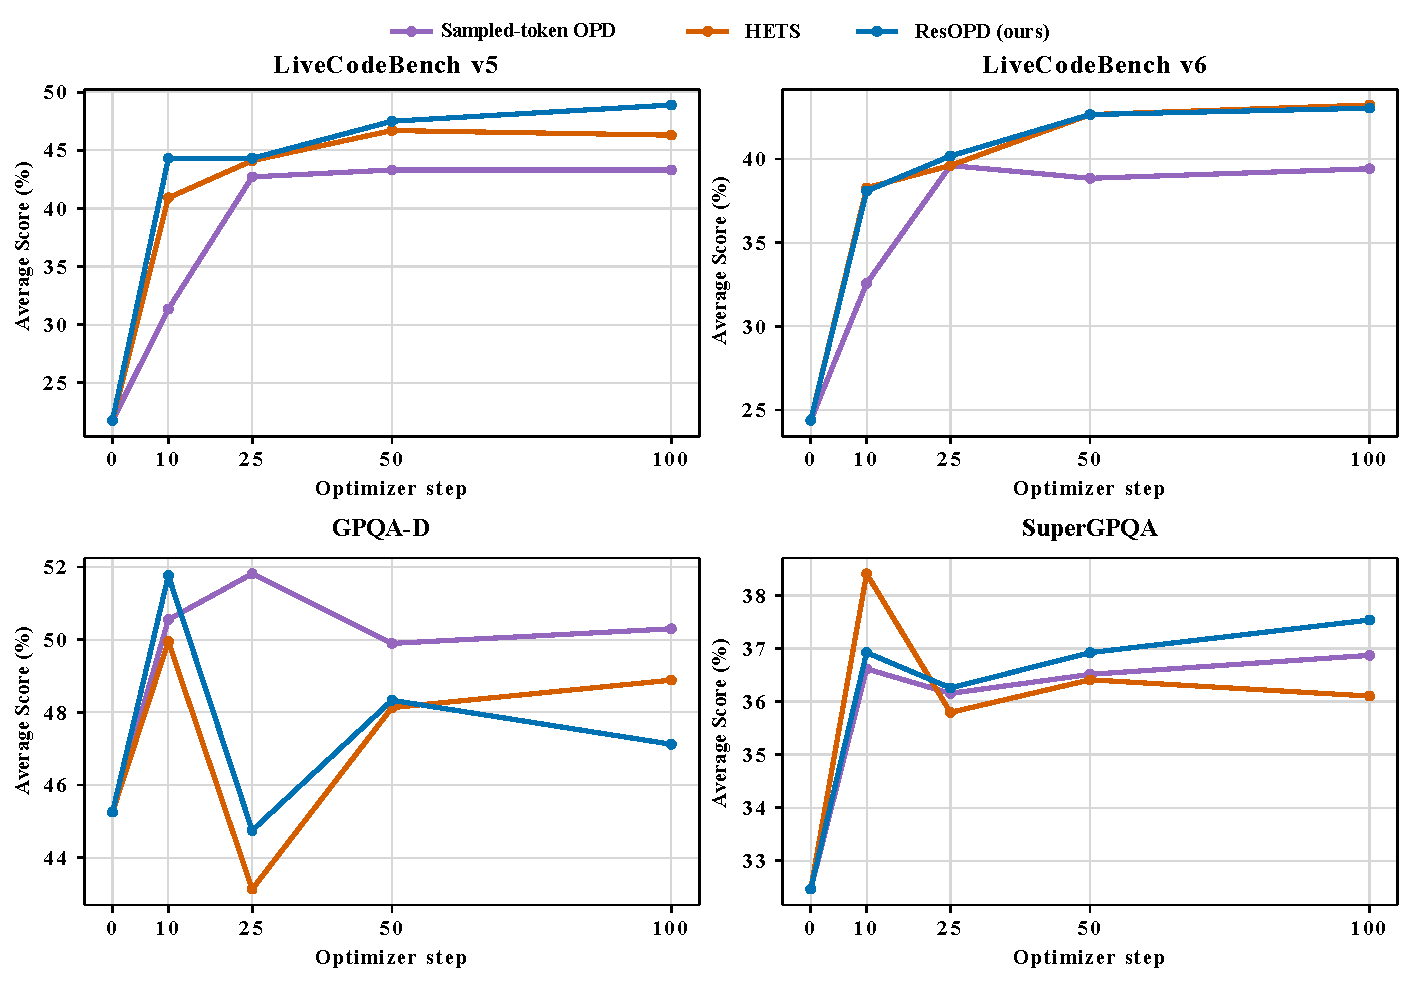
\includegraphics[width=0.85\columnwidth]{figs/qwen3_4b30_transfer_curves_v2.pdf}
    \caption{\textbf{从 Qwen3-30B-A3B-Instruct 到 Qwen3-4B 的跨领域蒸馏过程中的评估轨迹}，在优化器步骤（0、10、25、50 和 100）处。}
    \label{fig:qwen3-transfer-curves}
\end{figure}

\FloatBarrier
\section{诊断详情}
\label{app:math-curves}

\subsection{在线残余力矩测量}
\label{app:online-residual-moments}

在优化器更新 $u$ 时，令 $i \in \{1, \dots, B_u\}$  索引非空采样响应，$t \in \{1, \dots, T_{ui}\}$  索引其有效 token。我们定义标量支持残差及其组成部分为
\begin{equation}
  P_{uit} \coloneqq p_\theta(S_{uit} \mid x_{uit}), \qquad
  H_{uit} \coloneqq \ind\{A_{uit} \in S_{uit}\}, \qquad
  Z_{uit} \coloneqq H_{uit} - P_{uit}.
  \label{eq:online-support-residual}
\end{equation}
此处，$P_{uit}$ 表示分配给传输的教师模型 \text{Top-}$k$ 支持集 $S_{uit}$ 的学生模型概率质量，而 $H_{uit}$ 表示采样的学生 token 是否落入该集合。在确切的同策略采样下，残差条件期望为零，$\E[Z_{uit} \mid x_{uit}] = 0$ ，其条件方差为 $\E[Z_{uit}^2 \mid x_{uit}] = P_{uit}(1 - P_{uit})$ 。更一般地，其未中心化的二阶矩同时捕捉了内在采样变异性以及任何实现的校准漂移。

图~\ref{fig:training-dynamics-event-g0} 报告了该量的两种诊断聚合。面板~C 展示了掩码 token 级别的二阶矩：
\begin{equation}
  M_{2,\mathrm{tok}}^{(u)} = \frac{1}{\sum_{i=1}^{B_u} T_{ui}} \sum_{i=1}^{B_u} \sum_{t=1}^{T_{ui}} Z_{uit}^2,
  \label{eq:online-token-m2}
\end{equation}
而面板D通过先对每次反应内的数据求平均，再对各反应进行均匀加权，来评估轨迹层面的方差：
\begin{equation}
  \bar{Z}_{ui} = \frac{1}{T_{ui}} \sum_{t=1}^{T_{ui}} Z_{uit}, \qquad
  M_{2,\mathrm{traj}}^{(u)} = \frac{1}{B_u} \sum_{i=1}^{B_u} \bar{Z}_{ui}^2.
  \label{eq:online-trajectory-m2}
\end{equation}
直观上，$M_{2,\mathrm{tok}}$ 捕捉了未解析的头对尾事件的瞬时幅度（这在图~\ref{fig:topk-ablation} 中被用于近似事件间方差因子 $P\tau_p$），而 $M_{2,\mathrm{traj}}$ 则衡量了在序列滚动过程中持续存在的、带有符号的事件不平衡。定义批量均值 $\bar{Z}_u = B_u^{-1} \sum_{i=1}^{B_u} \bar{Z}_{ui}$ ，轨迹均值的经验标准差为
\begin{equation}
  \widehat{\operatorname{SE}}(\bar{Z}_u) = \sqrt{\frac{\max\{M_{2,\mathrm{traj}}^{(u)} - \bar{Z}_u^2, 0\}}{B_u - 1}}.
  \label{eq:online-trajectory-se}
\end{equation}

ResOPD 的连接在标量系数层面上是确切的。注意到尾部指标和尾部质量满足 $J_{uit} = 1 - H_{uit}$ 和 $\tau_{p,uit} = 1 - P_{uit}$ ，我们得到 $Z_{uit} = \tau_{p,uit} - J_{uit}$ 。将其代入式~(\ref{eq:residualization}) 得
\begin{equation}
  \widehat{\bgrad}_{uit}^{\mathrm{ResOPD}} - \widehat{\bgrad}_{uit}^{\mathrm{HETS}} = Z_{uit} \bmean_{B,uit}.
  \label{eq:online-residual-cfr-link}
\end{equation}
因此，这两个 $M_2$  指标直接追踪了随机标量对 ResOPD 桶控制幅度及其序列级持续性的调节。由于它们有意忽略了 $\lVert\bmean_{B,uit}\rVert$ 、其与细尾均值的对齐以及尾部内部的正交波动，因而作为计算轻量、机制对齐的在线诊断工具，而非完整的协方差估计量或固定前缀 NSR 的替代品。最后，尽管 $Z$  可以在稀疏的 Top-$k$  目标中被简单记录，但直接的 Top-$k$  rKL 缺乏采样尾部修正，且相对于真实 rKL 目标始终存在有偏性。因此，其零动作采样方差无法与图 C 和图 D 中无偏的 vOPD、HETS 以及 ResOPD 估计量相比较。


\subsection{有限梯度枚举检查}
\label{app:finite-check}

我们还在无蒙特卡罗误差的情况下，验证了四动作 Softmax 的无偏性恒等式。学生和教师的概率分别为 $(0.35,0.30,0.20,0.15)$ 和 $(0.60,0.25,0.10,0.05)$，前两个动作构成教师的 Top-2 支持集。我们直接对完整的反向 KL 散度进行微分，枚举每个可能的学生动作，并以其确切的学生动作概率加权估计量的梯度。所得的 HETS 期望与稠密全反向 KL 梯度的最大绝对误差为 $5.6\times10^{-17}$ 。

ResOPD 相对于 HETS 将逐动作向量改变了 $(\tau_p-J)\bmean_B$。由于相同的枚举具有 $\E[J]=\tau_p$，该修正的总和恰好为零，ResOPD 恢复了相同的稠密梯度。这种有限检查补充了公式~(\ref{eq:residualization}) 中的符号恒等式：它验证了停止系数和支持掩码的实现语义，但它并不是关于协方差或下游准确率的经验证据。

\subsection{完整的冻结前缀支持诊断}
\label{app:fixed-prefix-sweep}

\begin{table}[t]
\caption{\textbf{在固定教师模型 Top-$k$  输出负载下的支持集大小 ($k$ ) 检查。}
``移除的方差'' 表示相对于采样 token 的 OPD，经验协方差迹的减小量。负载包含 $k$  个 Top-$k$  项以及采样 token（各含 INT32 ID 和 FP32 概率对数）。学生质量与头部命中分别表示落在 Top-$k$  支持集中的预测概率和经验概率。各情景下最佳方差减小和 NSR 以 \textbf{粗体} 标出。}
\label{tab:fixed-prefix-sweep}
\centering
\small
\renewcommand{\arraystretch}{1.16}
\setlength{\tabcolsep}{4.0pt}

\begin{tabular*}{\textwidth}{@{\extracolsep{\fill}}lrrccrrrr@{}}
\toprule
\multirow{2}{*}{\shortstack[l]{Dataset \\ Student/Teacher}}
& \multirow{2}{*}{$k$}
& \multirow{2}{*}{\shortstack{Payload \\ (B/token)}}
& \multirow{2}{*}{\shortstack{Student \\ mass}}
& \multirow{2}{*}{\shortstack{Head \\ Hit}}
& \multicolumn{2}{c}{Var. Removed (\%) $\uparrow$}
& \multicolumn{2}{c}{NSR $\downarrow$} \\
\cmidrule(lr){6-7}\cmidrule(l){8-9}
& & & & & HETS & ResOPD & HETS & ResOPD \\
\midrule
\multirow{4}{*}{\shortstack[l]{\textbf{GSM8K} \\ 0.8B/4B}}
& 1  & 16  & $75.0\%$ & $74.8\%$  & $-0.5$ & $\mathbf{20.5}$ & 5.446 & $\mathbf{4.310}$ \\
& 4  & 40  & $93.1\%$ & $92.9\%$  & 27.3   & $\mathbf{52.5}$ & 3.940 & $\mathbf{2.573}$ \\
& 16 & 136 & $97.7\%$ & $97.9\%$  & 62.6   & $\mathbf{75.3}$ & 2.027 & $\mathbf{1.337}$ \\
& 64 & 520 & $99.3\%$ & $99.7\%$  & 85.1   & $\mathbf{89.5}$ & 0.807 & $\mathbf{0.570}$ \\
\addlinespace[0.25em]
\multirow{3}{*}{\shortstack[l]{\textbf{HMMT26} \\ 4B/27B}}
& 1  & 16  & $89.1\%$ & $89.3\%$   & $-1.0$ & $\mathbf{32.0}$ & 6.656 & $\mathbf{4.479}$ \\
& 4  & 40  & $99.1\%$ & $98.8\%$   & 55.8   & $\mathbf{75.3}$ & 2.914 & $\mathbf{1.630}$ \\
& 16 & 136 & $99.9\%$ & $100.0\%$  & 89.8   & $\mathbf{94.2}$ & 0.675 & $\mathbf{0.382}$ \\
\bottomrule
\end{tabular*}
\end{table}


\begin{figure}[t]
\centering
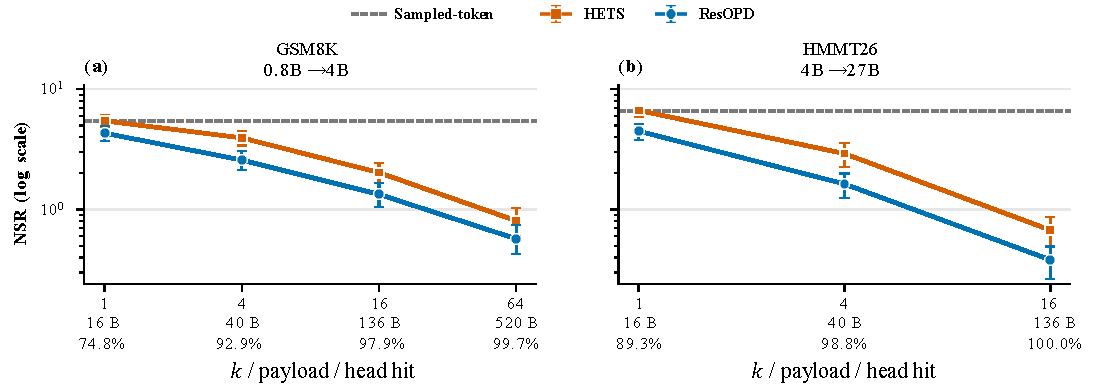
\includegraphics[width=0.96\textwidth]{figs/fixed_prefix_support_strata_v2.pdf}
\caption{\textbf{在基准测试中对冻结前缀支持大小（$k$）的全面诊断。} 
ResOPD 在 GSM8K 和 HMMT 上所有评估的支持大小下，持续降低了无量纲 NSR（对数尺度）。坐标轴标注详细说明了传输的教师端支持大小 $k$、相应的通信负载（字节/token）以及经验头部命中概率。误差条表示 95\% 轨迹级自助法置信区间。}
\label{fig:fixed-prefix-diagnostics}
\end{figure}

在表~\ref{tab:fixed-prefix-sweep} 中的两个测试套件中，ResOPD 在每个匹配的支持大小下均持续优于 HETS，实现了更高的协方差-迹消除和更低的 NSR。将 $k$ 从 $4$ 扩展到 $16$ 和 $64$ 会使传输成本分别增加 $3.4\times$ 和 $13\times$  ($40 \to 136 \to 520$ \,B/token)，但边际方差收益递减。关键的是，头部命中率表明仅高支持覆盖是不够的：即使头部质量达到 $98.8\%$  ($k=4$  on HMMT26)，稀有 $1.2\%$  尾部采样仍导致显著的 HETS--ResOPD 方差差距（$55.8\%$ 与 $75.3\%$  被消除）。此外，在 $k=1$ 处，HETS 表现出负向减少（$-1.0\%$ ），而 ResOPD 稳定地消除了 $32.0\%$  的梯度方差。这有力证实了公式~(\ref{eq:hets-cfr-variance-appendix}) 中的理论条件，确认尽管尾部采样的名义概率质量较低，但未校正的尾部采样仍主导残余梯度噪声。

\subsection{不同学习率下的训练动态}
\label{app:lr-sensitivity}


\paragraph{潜在的训练动态。}
图~\ref{fig:lr-sensitivity} 中的训练轨迹揭示了这种发散背后的两个清晰机制。首先，在梯度幅值方面，ResOPD 在 $5\times10^{-6}$ 时保持显著更低的裁剪前梯度范数（均值 $0.43$  vs.\ $0.48$ ；99\%分位数 $0.97$  vs.\ $1.84$ ），且完全避免了梯度裁剪（$0/64$  步 vs.\ $2/64$  步，对应 HETS）。其次，在残差稳定化方面，图 (B)--(D) 显示，ResOPD 一致地抑制了支持集质量差距 ($Q-P$ )，并压制了 token 级和轨迹级残差二阶矩 ($M_2$ )，这与该步长下观察到的更稳定的学习轨迹一致。

\begin{figure}[t]
  \centering
  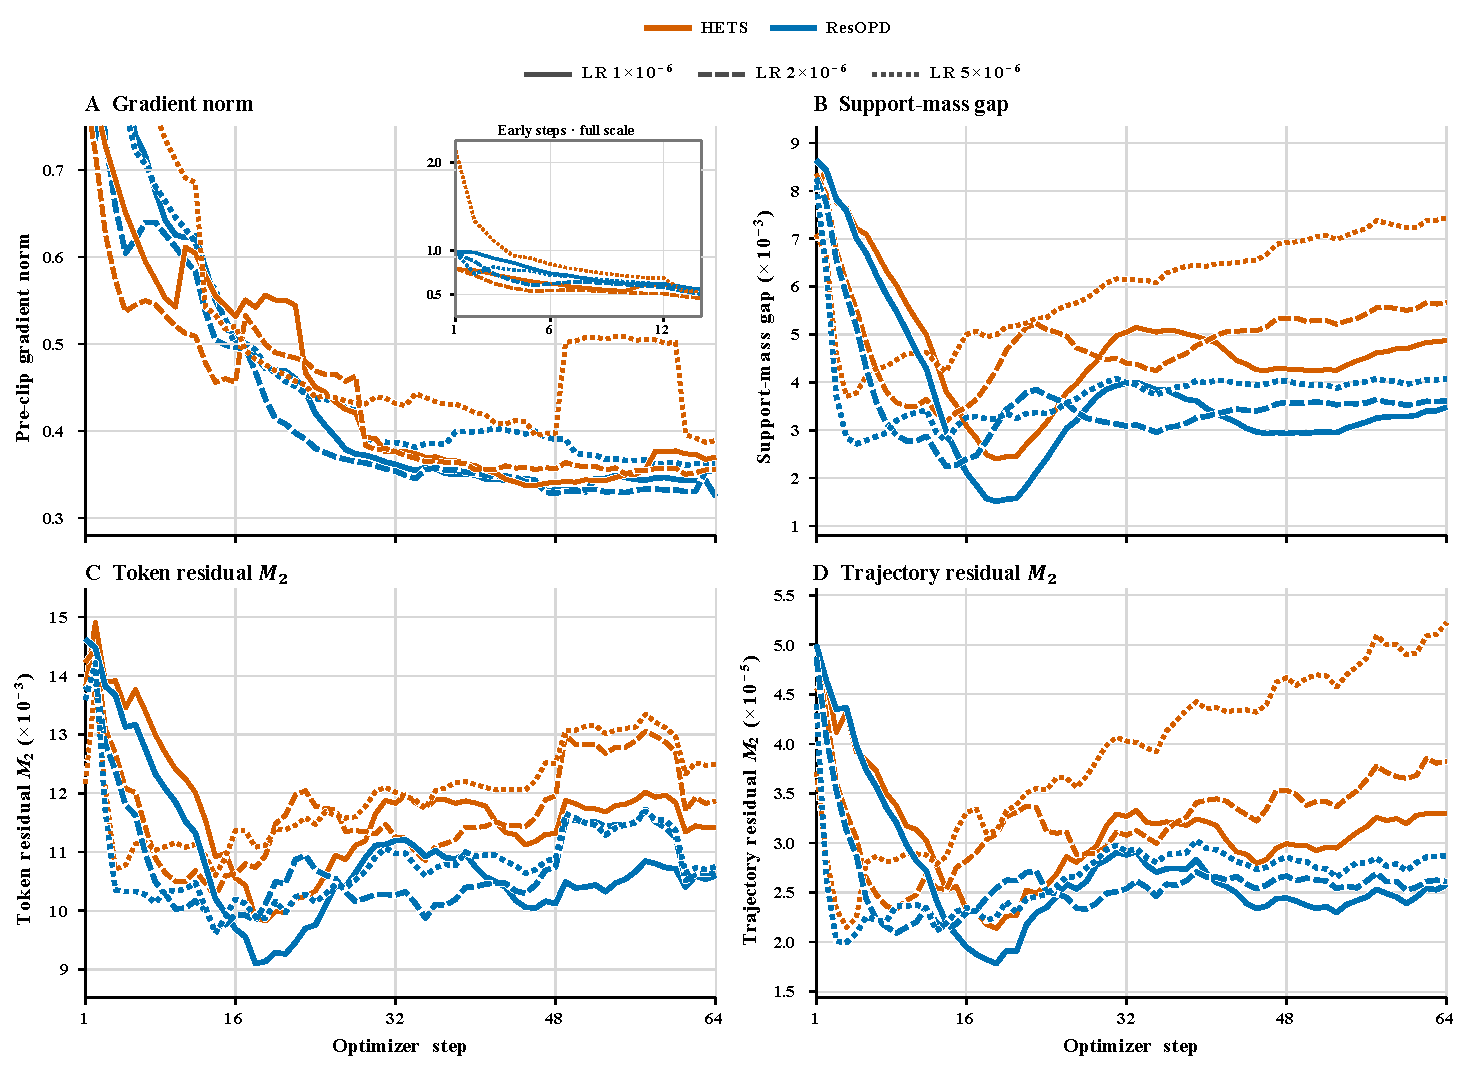
\includegraphics[width=0.9\columnwidth]{figs/lr_training_dynamics_cfr_v3.pdf}
  \caption{\textbf{训练动态与学习率敏感性}：HETS (\textit{橙色}) 与 ResOPD (\textit{蓝色}) 在 DeepMath 上的对比，涵盖三个学习率（$1\times10^{-6}$ 实线，$2\times10^{-6}$ 虚线，$5\times10^{-6}$ 点划线）。
\textbf{(A)} 截断前的全局梯度范数（插图显示早期步骤中完整未截断峰值的全尺度情况）。
\textbf{(B)} 传输教师 Top-4 token 的支持质量差 ($Q - P$ )。
\textbf{(C, D)} token 级别与轨迹级别的二阶残差矩 ($M_2$ )。
当学习率提升至 $5\times10^{-6}$ 时，HETS 表现出显著的梯度范数波动以及逐渐增大的质量/残差差异，而 ResOPD 则保持稳定的动态，并在整个最优化过程中始终贴近其低学习率轨迹。}
  \label{fig:lr-sensitivity}
\end{figure}